% IEEE standard conference template; to be used with:
%   spconf.sty  - LaTeX style file, and
%   IEEEbib.bst - IEEE bibliography style file.
% --------------------------------------------------------------------------

\documentclass[letterpaper]{article}
\usepackage{spconf,amsmath,amssymb,graphicx,listings,hyperref,array,float,epstopdf}
\lstset{basicstyle=\ttfamily\footnotesize,numbers=left,stepnumber=2,frame=single,language=c,captionpos=b}
\usepackage[utf8]{inputenc} % UTF-8 was invented to be used.

% Example definitions.
% --------------------
% nice symbols for real and complex numbers
\newcommand{\R}[0]{\mathbb{R}}
\newcommand{\C}[0]{\mathbb{C}}



% bold paragraph titles
\newcommand{\mypar}[1]{{\bf #1.}}
 
% Title.
% ------
\title{How to write a fast Optimal Binary Search Tree Implementation}
%
% Single address.
% ---------------
\name{Jeremia Bär, Stefan Dietiker\thanks{The author thanks Jelena
    Kovacevic. This paper is a modified version of the template she
    used in her class.}}  \address{Department of Computer
  Science\\ ETH Z\"urich\\Z\"urich, Switzerland}

% For example:
% ------------
%\address{School\\
%		 Department\\
%		 Address}
%
% Two addresses (uncomment and modify for two-address case).
% ----------------------------------------------------------
%\twoauthors
%  {A. Author-one, B. Author-two\sthanks{Thanks to XYZ agency for funding.}}
%		 {School A-B\\
%		 Department A-B\\
%		 Address A-B}
%  {C. Author-three, D. Author-four\sthanks{The fourth author performed the work
%		 while at ...}}
%		 {School C-D\\
%		 Department C-D\\
%		 Address C-D}
%

\DeclareMathOperator{\depth}{depth}

\begin{document}
%\ninept
%
\maketitle
%

\begin{abstract}
	We were able to show that with simple changes to the program structure,
	blabla.
\end{abstract}


\section{Introduction}\label{sec:intro}
Search trees are among the most fundamental, if not the most fundamental, data
structure known in computer science. 

Given the simple and recursive structure of a binary search tree, it is easy to
deduce an algorithm to find a specific key in the tree. However, as every binary
search tree can be restructured arbitrarily yielding a new valid binary search
tree holding the same set of keys and, in general, there are great variances
among these tree structures concerning the lookup cost, the ``naked''
binary search tree must be accompanied by an algorithm, the sophistication of
which lies in its capability to structure the tree optimally with respect to the
lookup cost.

For dynamic binary search trees, various algorithms have been developed to
balance the tree on inseration and deletion (references). In the case of static
binary search trees, on the other hand, the set of keys is given a priori, along
with a probability distribution that indicates the likeliness of an individual
key being searched for. Based upon this, one can construct an optimal binary
search tree, that is, a search tree which has a minimal expected lookup cost.

In the following we introduce a dynamic programming algorithm, which solves the
problem by examining combinations of optimal subtrees. Our objective then is to
optimally implement this algorithm on a modern Intel-based hardware platform.

Our interest in this algorithm emerges from its straight-forward design which,
not only makes its own algorithmic properties apparent and easy to analyze, but
also provides us with clear conceptual guidance when optimizing the algorithm.
Our hope is thus that the observations made in this report can be translated to
similar problems.

\section{Background}

As a group we worked on the static optimal binary search tree problem.
In this section we give a mathematical description of the optimal binary
search tree problem. The algorithm implemented and optimized to solve the
problem is presented and a cost measure introduced. The presentation is
based on the algorithms book by Cormen et al.~\cite{MITBook}. We conclude
by giving a short overview of two asymptotically faster algorithms.

\mypar{Problem Statement} Let $K = \{k_1, k_2, \dots, k_n\}$ be a sequence
of distinct ordered keys. For each key $k_i$, let $p_i$ be the probability
that a given search is for key $k_i$. Such a search is called successfull.
Furhter, let $D = \{d_0, d_1, \dots, d_n\}$ be the set of dummy keys
returned for unsuccessfull searches as follows: $d_i$ represents searches
for values between $k_i$ and $k_{i+1}$, $d_0$ represent the values smaller
$k_0$ and $d_n$ the values larger $k_n$. For each dummy key $d_i$, let
$q_i$ be the probability that a given search returns $d_i$.
A valid solution to the static binary search tree problem is any binary
search tree $T$ that has $K$ as nodes and $D$ as leaves.
The cost of a search in a such a tree $T$ is defined as the depth of the key
found plus one. Since $K$ and $D$ cover all possible searches,
$\sum_{i=1}^n p_i + \sum_{j=0}^n q_j = 1$ and we can compute the expected
cost of a search in $T$ as:
\begin{align}
  %\mathbb{E}[\text{search cost in } T] =
  %\nonumber\\
  %\mathcal{E}_T &=
  \sum_{i=1}^n (\depth_T(k_i) + 1) \cdot p_i
   + \sum_{i=0}^n (\depth_T(d_i) + 1) \cdot q_i
  \nonumber\\
  % I just can't fit the formula to width :-(
  = 1 + \sum_{i=1}^n \depth_T(k_i) \cdot p_i
      + \sum_{i=0}^n \depth_T(d_i) \cdot q_i
  \label{eqn:cost}
\end{align}
A static binary search tree is called optimal if its expected search cost
is minimal amongst all valid solution trees.
We can now formulate the static optimal binary search tree problem as
follows: Given $K$, $P$ and $Q$, find the optimal binary search tree.

\mypar{Algorithm} Devising an algorithm to solve the problem requires a
crucial insight on the problem structure: Given an optimal tree $T$ for
keys $k_1$ to $k_n$ with root $k_r$, its left subtree $T_L$ is an optimal
solution for the keys $k_1$ to $k_{r-1}$. Clearly, it has to be a binary
search tree for these keys. Then, if it were not optimal, one could replace
$T_L$ by an optimal binary search tree for the keys $k_1,\dots,k_{r-1}$
obtaining a better solution $T'$ for the original problem. However, this
contradicts the optimality of $T$ and hence $T_L$ is optimal as well. This
argument holds anologous for all subtrees in $T$.

From this insight we can construct an algorithm. Let $e[i,j]$ denote the
expected search cost in the optimal binary search tree continaing keys
$k_i$ through $k_j$. If such a tree is used as a left or right subtree to
construct a tree containing more keys, the depth of its nodes increases by
one. Following \autoref{eqn:cost}, the subtree's expected search cost
increases by
\begin{align}
  w(i,j) &= \sum_{l=1}^j p_l + \sum_{l=i-1}^j q_l \nonumber\\
         &= w(i,r-1) + p_r + w(r+1,j)
  \label{eqn:w}
\end{align}
where the second expression reflects the recursive structure of the problem
again. This allows to express the search cost of a binary search tree over
$k_i$ to $k_j$ with root $k_r$ constructed from its subtrees as
\begin{align}
  e[i,j] = e[i,r-1] + e[r+1,j] + w(i,j)
  \label{eqn:e-intermediate}
\end{align}
Knowing the optimal expected search costs for all possible subtrees, we can
construct the optimal binary search tree by choosing the key as root that
minimizes \autoref{eqn:e-intermediate}, i.e
\footnote{Note that for simplicity, we do not include border cases here.
For a complete discussion of the algorithm and its mathematics refer to
\cite{MITBook}.}
\begin{align}
  e[i,j] = \min_{i\leq r\leq j} \{e[i,r-1] + e[r+1,j] + w(i,j)\}
  \label{eqn:e}
\end{align}
This expression can now direclty be translated into code, as is shown in
\autoref{lst:baseline}. The cost of the subtrees is computed using dynamic
programming. The table \texttt{e[IDX(i,j)]} is used to store the
expected search cost for the optimal search tree covering keys in $k_i$
through $k_j$\footnote{Note that the code actually uses zero-indexing.}. We
fill the table \texttt{e} diagonal by diagonal. This corresponds to
computing first all the subrees continaing one key, then containing two
keys and so forth, as indicated by the length variable \texttt{l}. The
innermost \texttt{r}-loop iterates over all valid roots for the subtree to
find the optimal binary search tree for the current keys. We refer to the
expected cost \texttt{e[IDX(i,j)]} to be computed as the \emph{target
cell}. A second table called \texttt{root} is used to keep track which root
was chosen for the current subtree to be able to reconstruct the overall
optimal tree in the end. In the code section, we have omitted the
initialization code. The computation is dominated by the triple loop shown.
\begin{lstlisting}[
  caption={Basline Implementation},
  label=lst:baseline,
  float
]
for (l = 1; l < n+1; l++)
  for (i = 0; i < n-l+1; i++)
    j = i+l;
    e[IDX(i,j)] = INFINITY;
    w[IDX(i,j)] = w[IDX(i,j-1)] + p[j-1] + q[j];
    for (r = i; r < j; r++ )
      t = e[IDX(i,r)] + e[IDX(r+1,j)]
          + w[IDX(i,j)];
      if (t < e[IDX(i,j)])
        e[IDX(i,j)]    = t;
        root[IDX(i,j)] = r;
\end{lstlisting}

\mypar{Cost Analysis} The presented algorithm has runtime $O(n^3)$. As can
be seen in \autoref{lst:baseline}, the computation involves additions and
comparisions only. We define the cost function of the algorithm as the
number of floating point additions and floating point comparisons:
\begin{align*}
C(n) = (\#\text{adds}(n), \#\text{comps}(n))
\end{align*}
The body of the second loop is executed a total of
\begin{align*}
\sum_{i=1}^{n} i = \frac{n(n+1)}{2}
\end{align*}
times. The body of the innermost loop is executed a total of
\begin{align*}
\sum_{i=1}^{n} l\cdot(n-l) = \frac{1}{6}(n^3-n)
\end{align*}
times.  Hence, the cost function is defined as:
\begin{align*}
C(n) = \left(\frac{1}{3}(n^3+3n^2+2n), \frac{1}{6}(n^3 - n)\right)
\end{align*}

\mypar{Alternative Algorithms}
Knuth's better solution
O(1) algorithm

\section{Optimization}
In the following, we present the methods we used to gradually improve the
performance of the algorithm. We name the different implementations that we
obtained according to the methods we employed. Alongside the presented
methods, we also applied basic block optimizations such as scalar
replacement, strength reduction and loop unrolling. \autoref{fig:DecTree}
gives an overview of the optimizations applied.

\begin{figure}[htb]

\begin{center}
\begin{tikzpicture}[-,shorten >=1pt,auto,node distance=1.8cm,
  thick,main node/.style={font=\sffamily\scriptsize\bfseries}]
	
  \node[main node] (0) {Baseline};
  \node[main node] (1) [below=1em of 0] {Transposed};
	\node[main node] (2) [below=1em of 1] {Bottom-Up};
	\node[main node] (3) [below=1em of 2] {Partial-Results};
	\node[main node] (4) [below left=1em and 1em of 3] {Triangular};
	\node[main node] (5) [below=1em of 4] {Vectorized, Triangular};
	\node[main node] (6) [below right=1em and 1em of 3] {Blocking};
	\node[main node] (7) [below=1em of 6] {Vectorized, Blocking};

  \path[every node/.style={font=\sffamily\small}]
	(0) edge node [below] {} (1)
	  (1) edge node [below] {} (2)
		(2) edge node [below] {}(3)
		(3) edge node [below] {}(4)
		(4) edge node [below] {}(5)
		(3) edge node [below] {}(6)
		(6) edge node [below] {}(7)
		;
\end{tikzpicture}
\end{center}
\caption{Overview of optimizations.}
\label{fig:DecTree}
\end{figure}

\begin{figure}[htb]\centering
	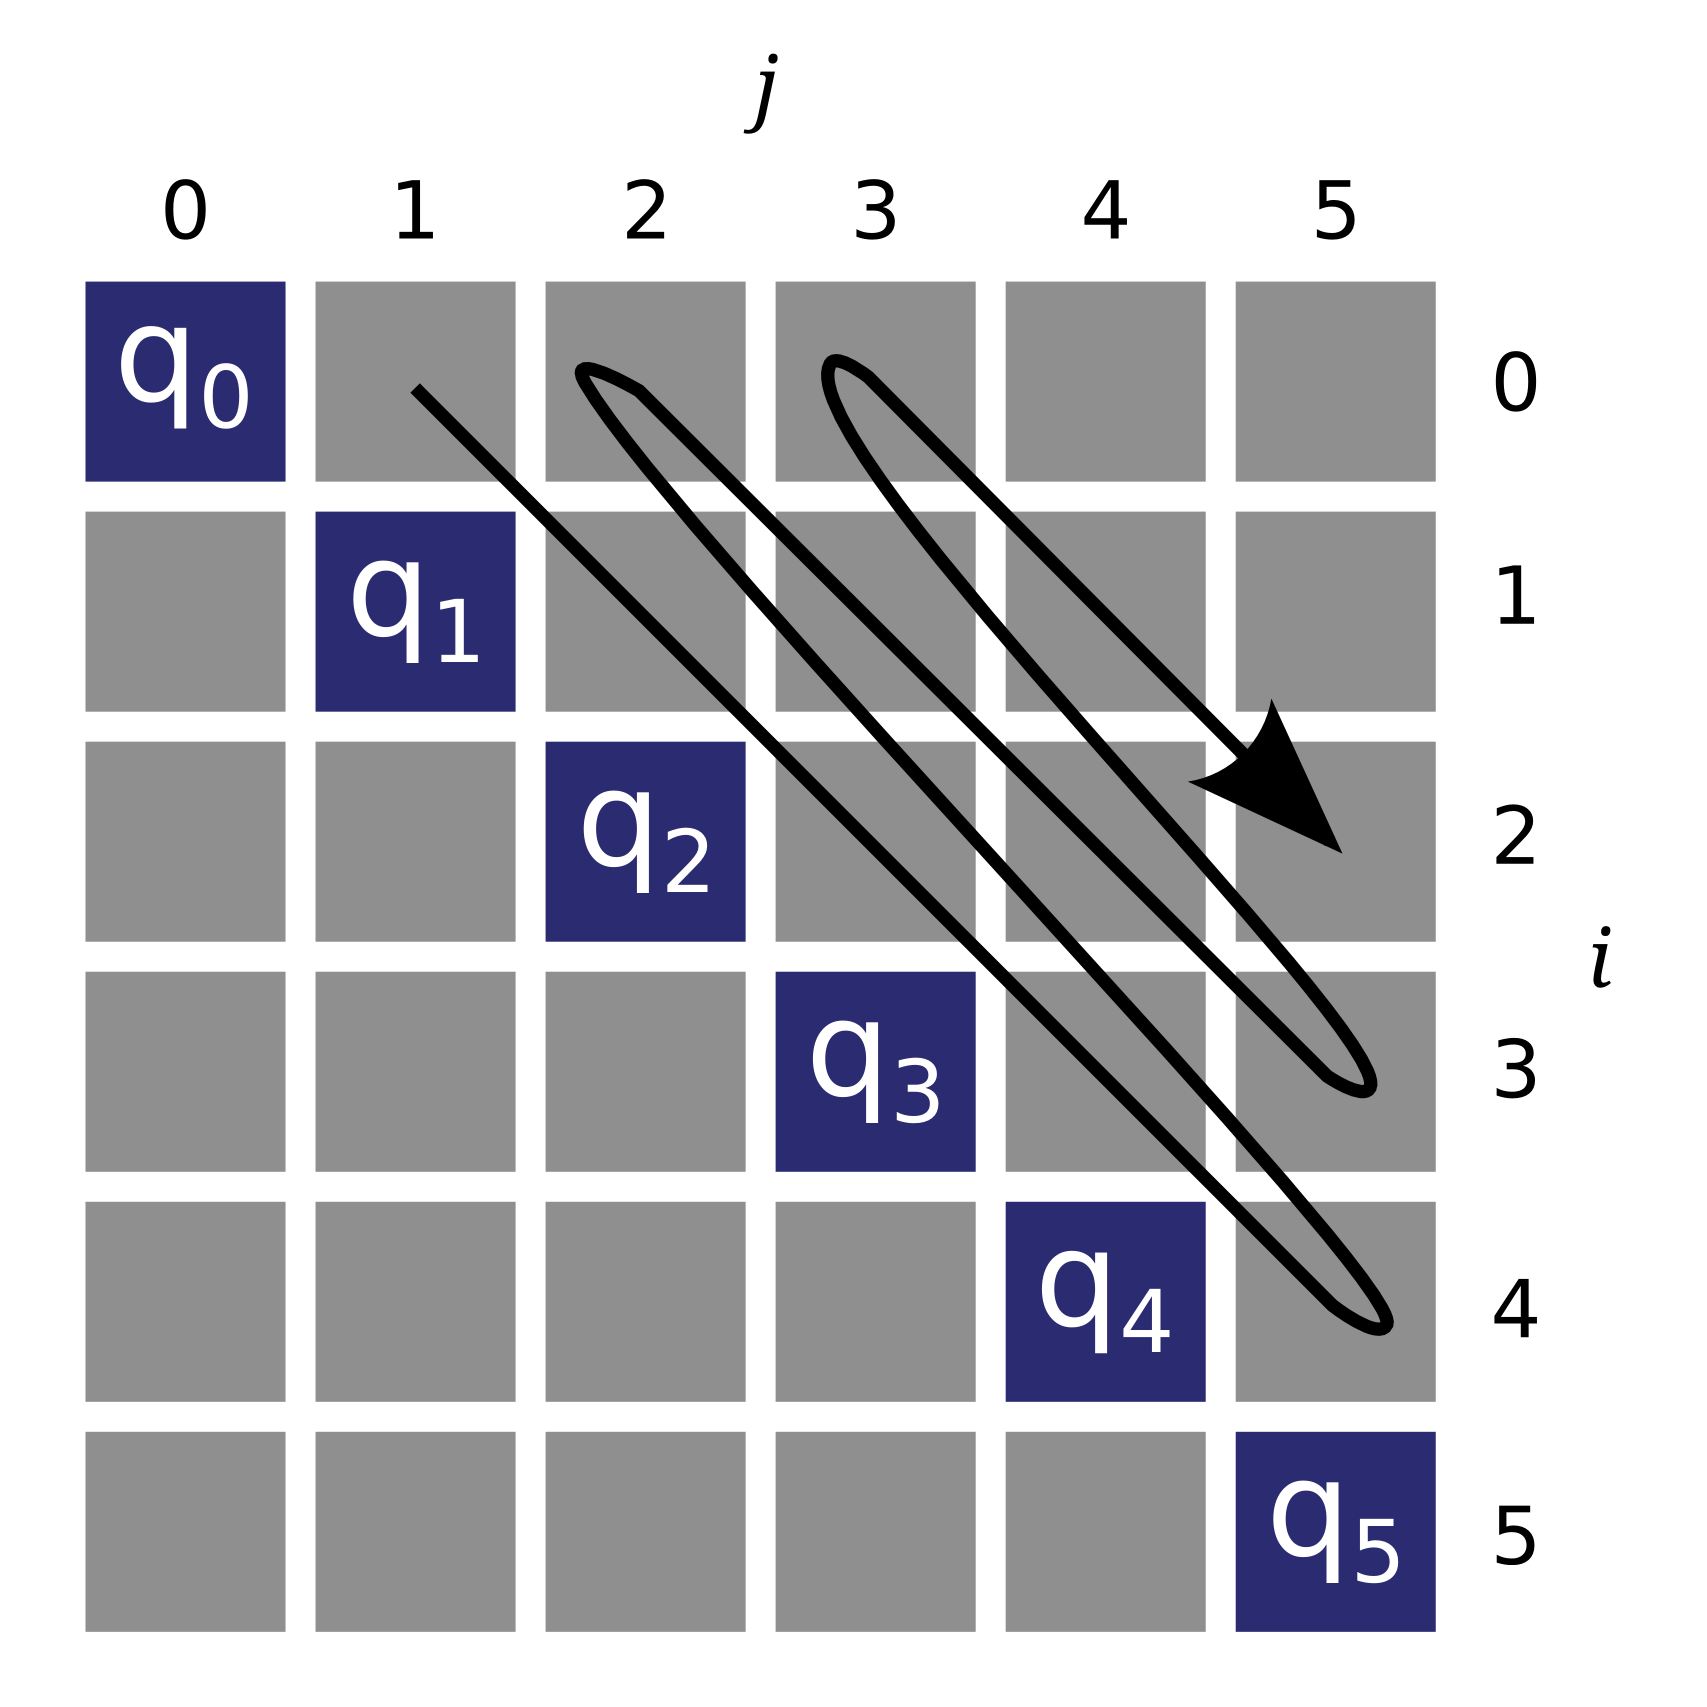
\includegraphics[width=0.33\textwidth]{img/reference_access.png}
  \caption{Access Pattern of reference implementation.\label{fig:reference}}
\end{figure}

\mypar{Transposed} Examining the innermost loop, we see that the table is
accessed row- and column-wise. Thus, the memory is accessed in strides of $1$
and $n+1$, respectively. However, with two simple changes to the algorithm, we
can avoid strides of $n+1$ and replace them with accesses of stride $1$: We make
use of the lower half of the square table in that we store newly calculated
values not only at $(i,j)$ but also at $(j,i)$. That is, instead of accessing a
column in the upper half, we access a row in the lower-half. This needs only two
minor changes to the algorithm as described in \autoref{lst:baseline}:
First, line $7$ turns into
\begin{center}
\verb:t = e[IDX(i,r)] + e[IDX(j,r+1)]:, 
\end{center}
and after line $10$, we would insert 
\begin{center}
	\verb:e[IDX(j,i)] = t;:.
\end{center}

\mypar{Bottom-Up} The order in which individual values are calculated is
along the diagonals, as visualized in Figure \ref{fig:reference}. We notice
that, for two distinct cells on a diagonal, their corresponding rows and
columns intersect exactly in one cell. By changing the outermost two loops
determining the target cell such that the table is built up row-wise and
bottom-up, as visualized in Figure \ref{fig:bottom-up}, we can improve
temporal locality with respect to the accesses to the row that is currently
being built-up.

\begin{figure}[htb]\centering
	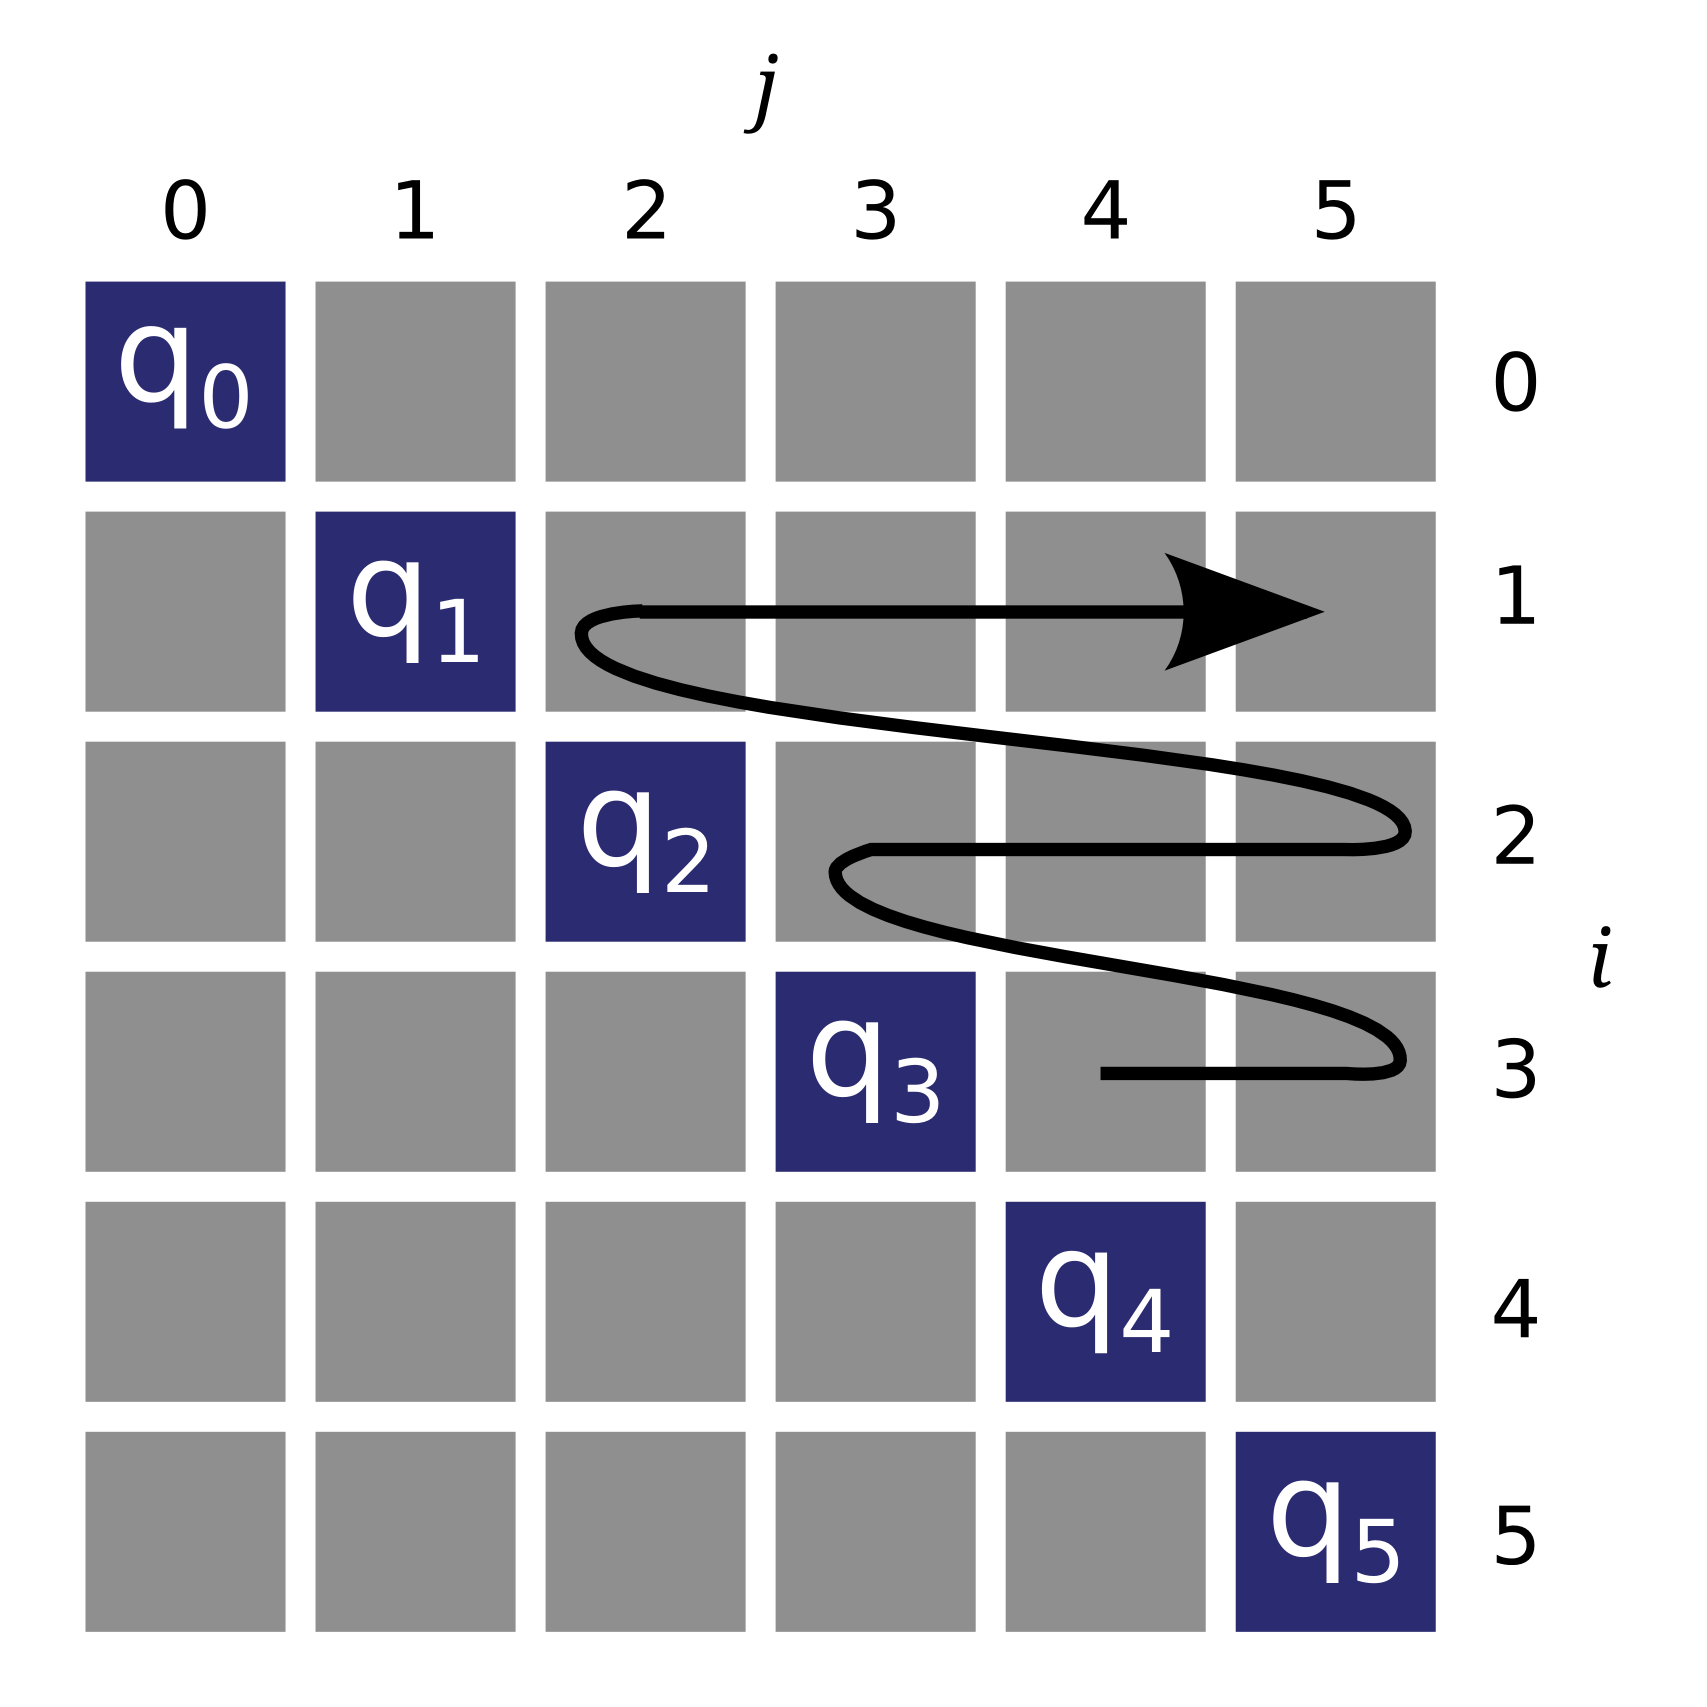
\includegraphics[width=0.33\textwidth]{img/bottom_up_access.png}
  \caption{Access Pattern of Bottom-Up.\label{fig:bottom-up}}
\end{figure}

\mypar{Partial Results} Instead of calculating the minimum value over a full row
and column, we can store intermediate values for an entire row by swapping the
innermost two loops. That is, for row $i$, we add the value $e[i,r], i\leq r\leq
n$ to all entries $e[r,j], r\leq j \leq n$ and store the minimum of that sum and
$e[i,r]$ in $e[i,r]$. \autoref{fig:partial} visualizes the pattern for one
consecutive executions of the $r$-loop (which is now the second innermost loop):
the value contained in the cell with the unfilled circle is added to all values
contained in the cells with the filled circle and the minimum is stored in the
white cells. This allows to have sequential access in the innermost loop
without the need to keep the transposed version of the data values in the
lower left half of the triangle.

\begin{figure}[htb]\centering
	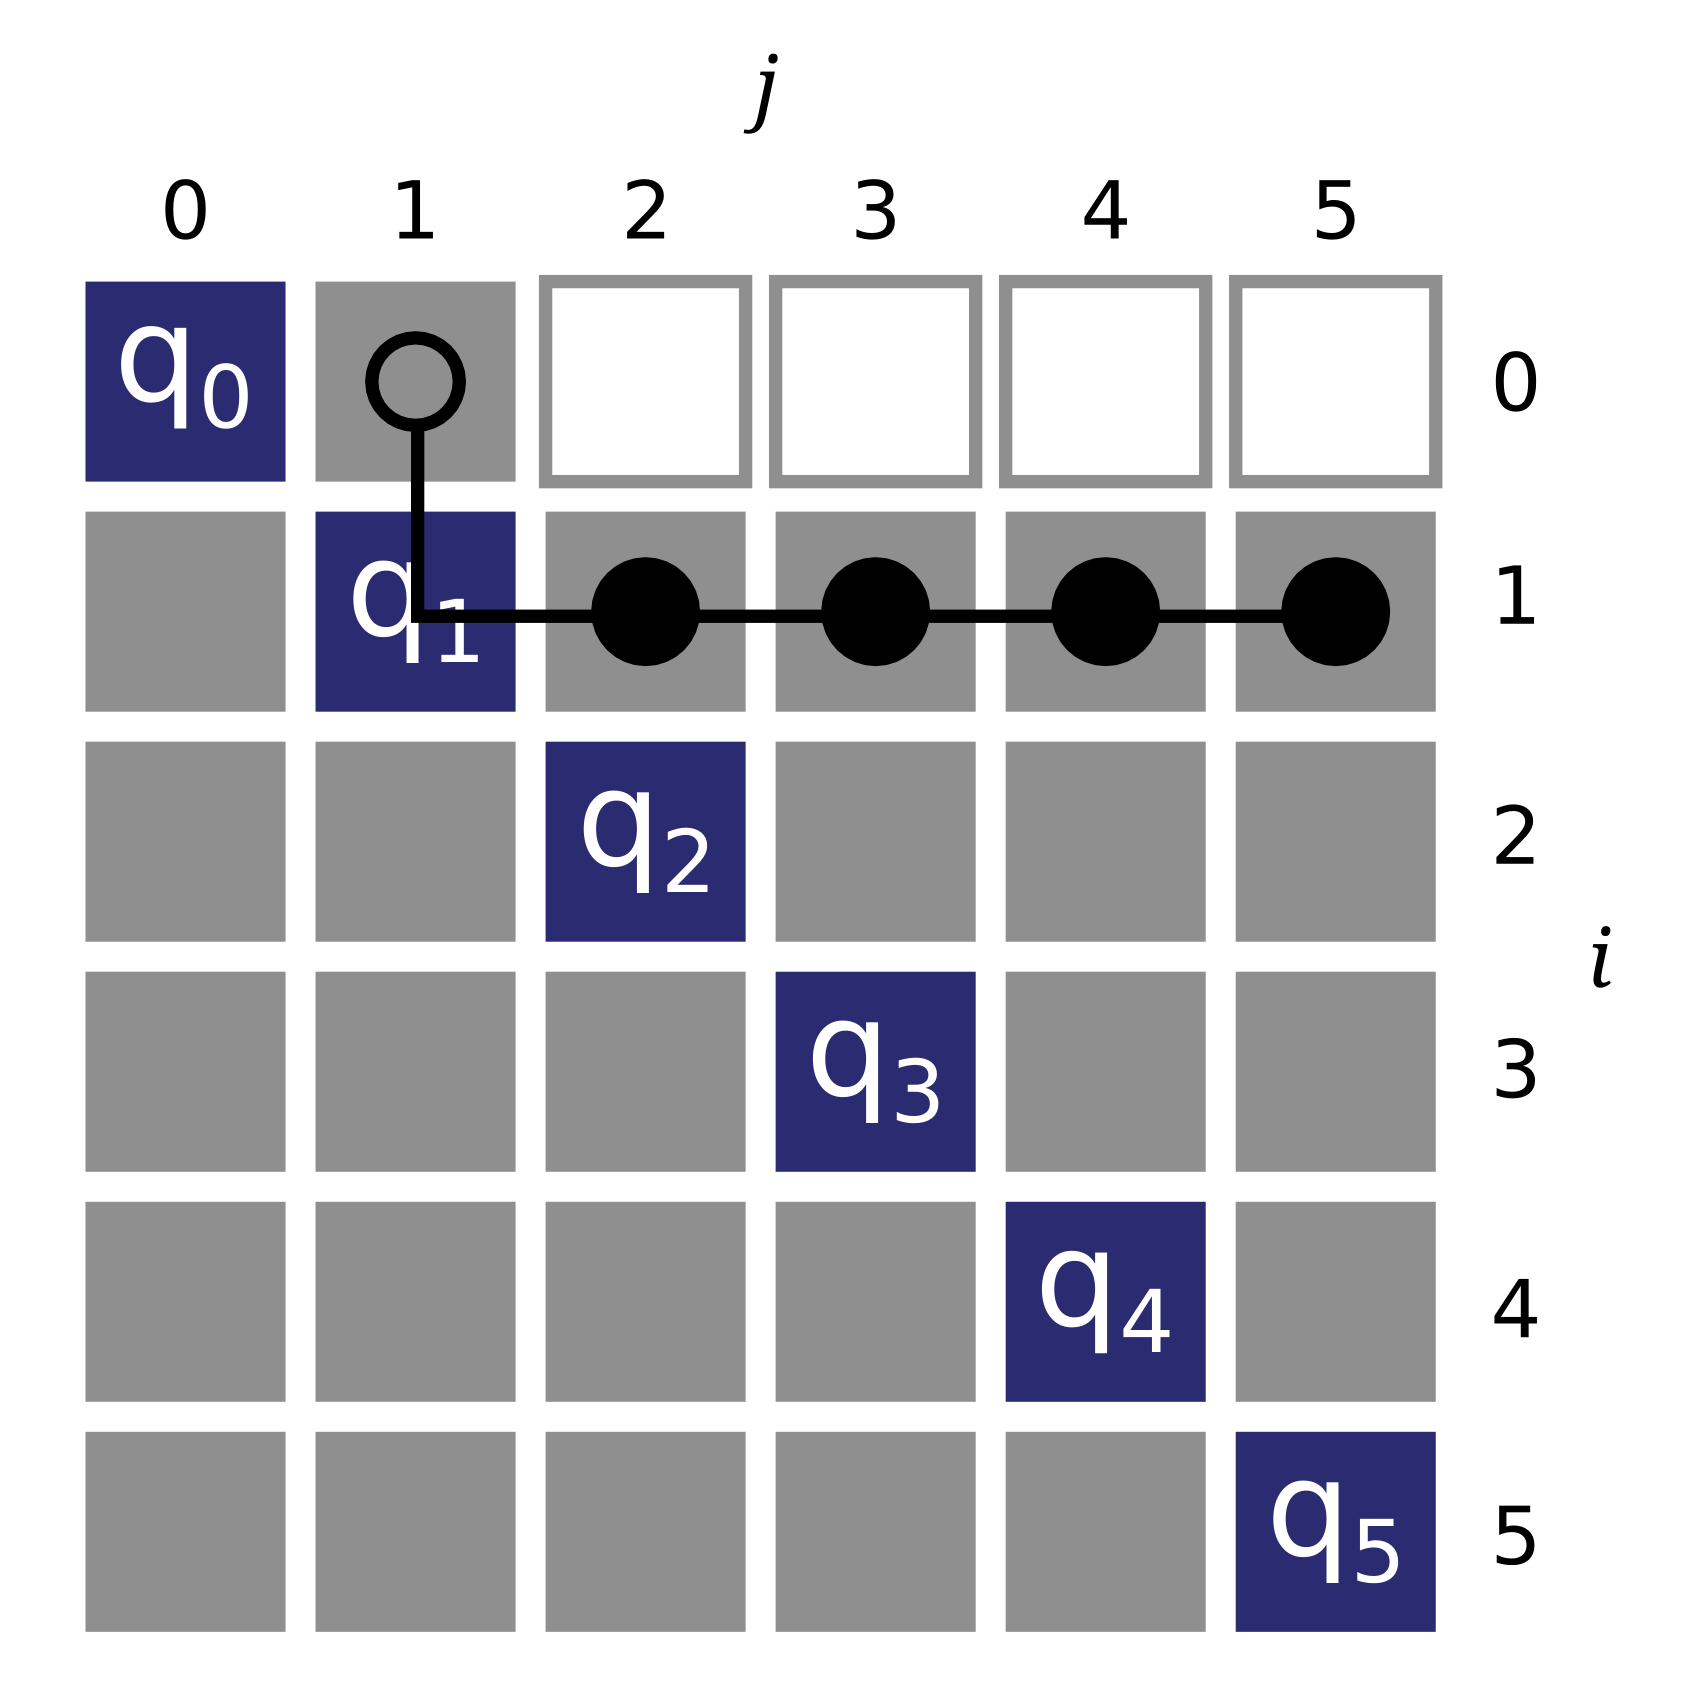
\includegraphics[width=0.33\textwidth]{img/intermediate_access.png}
  \caption{Storing Partial results.\label{fig:partial}}
\end{figure}

\mypar{Triangular} While the above approach need not necessarily improve
the performance over the \emph{Bottom Up}-approach, allocating the full
square memory is no longer required. We can \emph{compress} the memory
layout by concatenating the rows of the ``upper'' triangular table.  As for
each target row $i$ we compute, the full triangle below it is accessed row
after row, this yields unit stride access even at the end of each
intermediate row being traversed. The unused sections between the left end
of the square and the beginning of the triangle is now omitted. This
potentially also improves the performance of the hardware prefetcher. We
call this memory layout \emph{triangular}--as opposed to the \emph{square}
layout.

Using this memory layout significantly complicates the index calculation.
The correct index-macro for this memory layout is:
\begin{center}
	\scriptsize
	\begin{verbatim}#define IDX(i,j)\
	((n+1)*(n+2)/2 - (n-(i)+1)*(n-(i)+2)/2 + (j) - (i))\end{verbatim}
\end{center}
Strength reduction can be applied to alleviate the computation. Index
variables with constant offset changes over loop iterations make the
involved index computation obsolete.

\mypar{Vectorized Triangular} Historically, our initial approaches at
blocking, explained below, were unsuccessful. Thus, we focused on
vectorizing the triangular layout, which is straight-forward: The current
row is processed until the number of remaining cells is a multiple of the
vector length. From then on, vector instructions are used.

\mypar{Blocking} Based upon our \emph{Partial Results} approach, we employed a
blocking strategy as follows: We unrolled the two innermost loops.
Thus, instead of storing the partial results in the target row for each
subsequent row, we store calculate the minimum across multiple subsequent rows
before storing the result.
Figure \ref{fig:vec-blocking} visualizes the approach: The value stored in the
cell with the unfilled circle is added to the corresponding values stored in the
cells containing the filled circles. The minimum across the columns containing
the filled circles is stored in the empty cells which therefore contain partial
results.

\begin{figure}[htb]\centering
	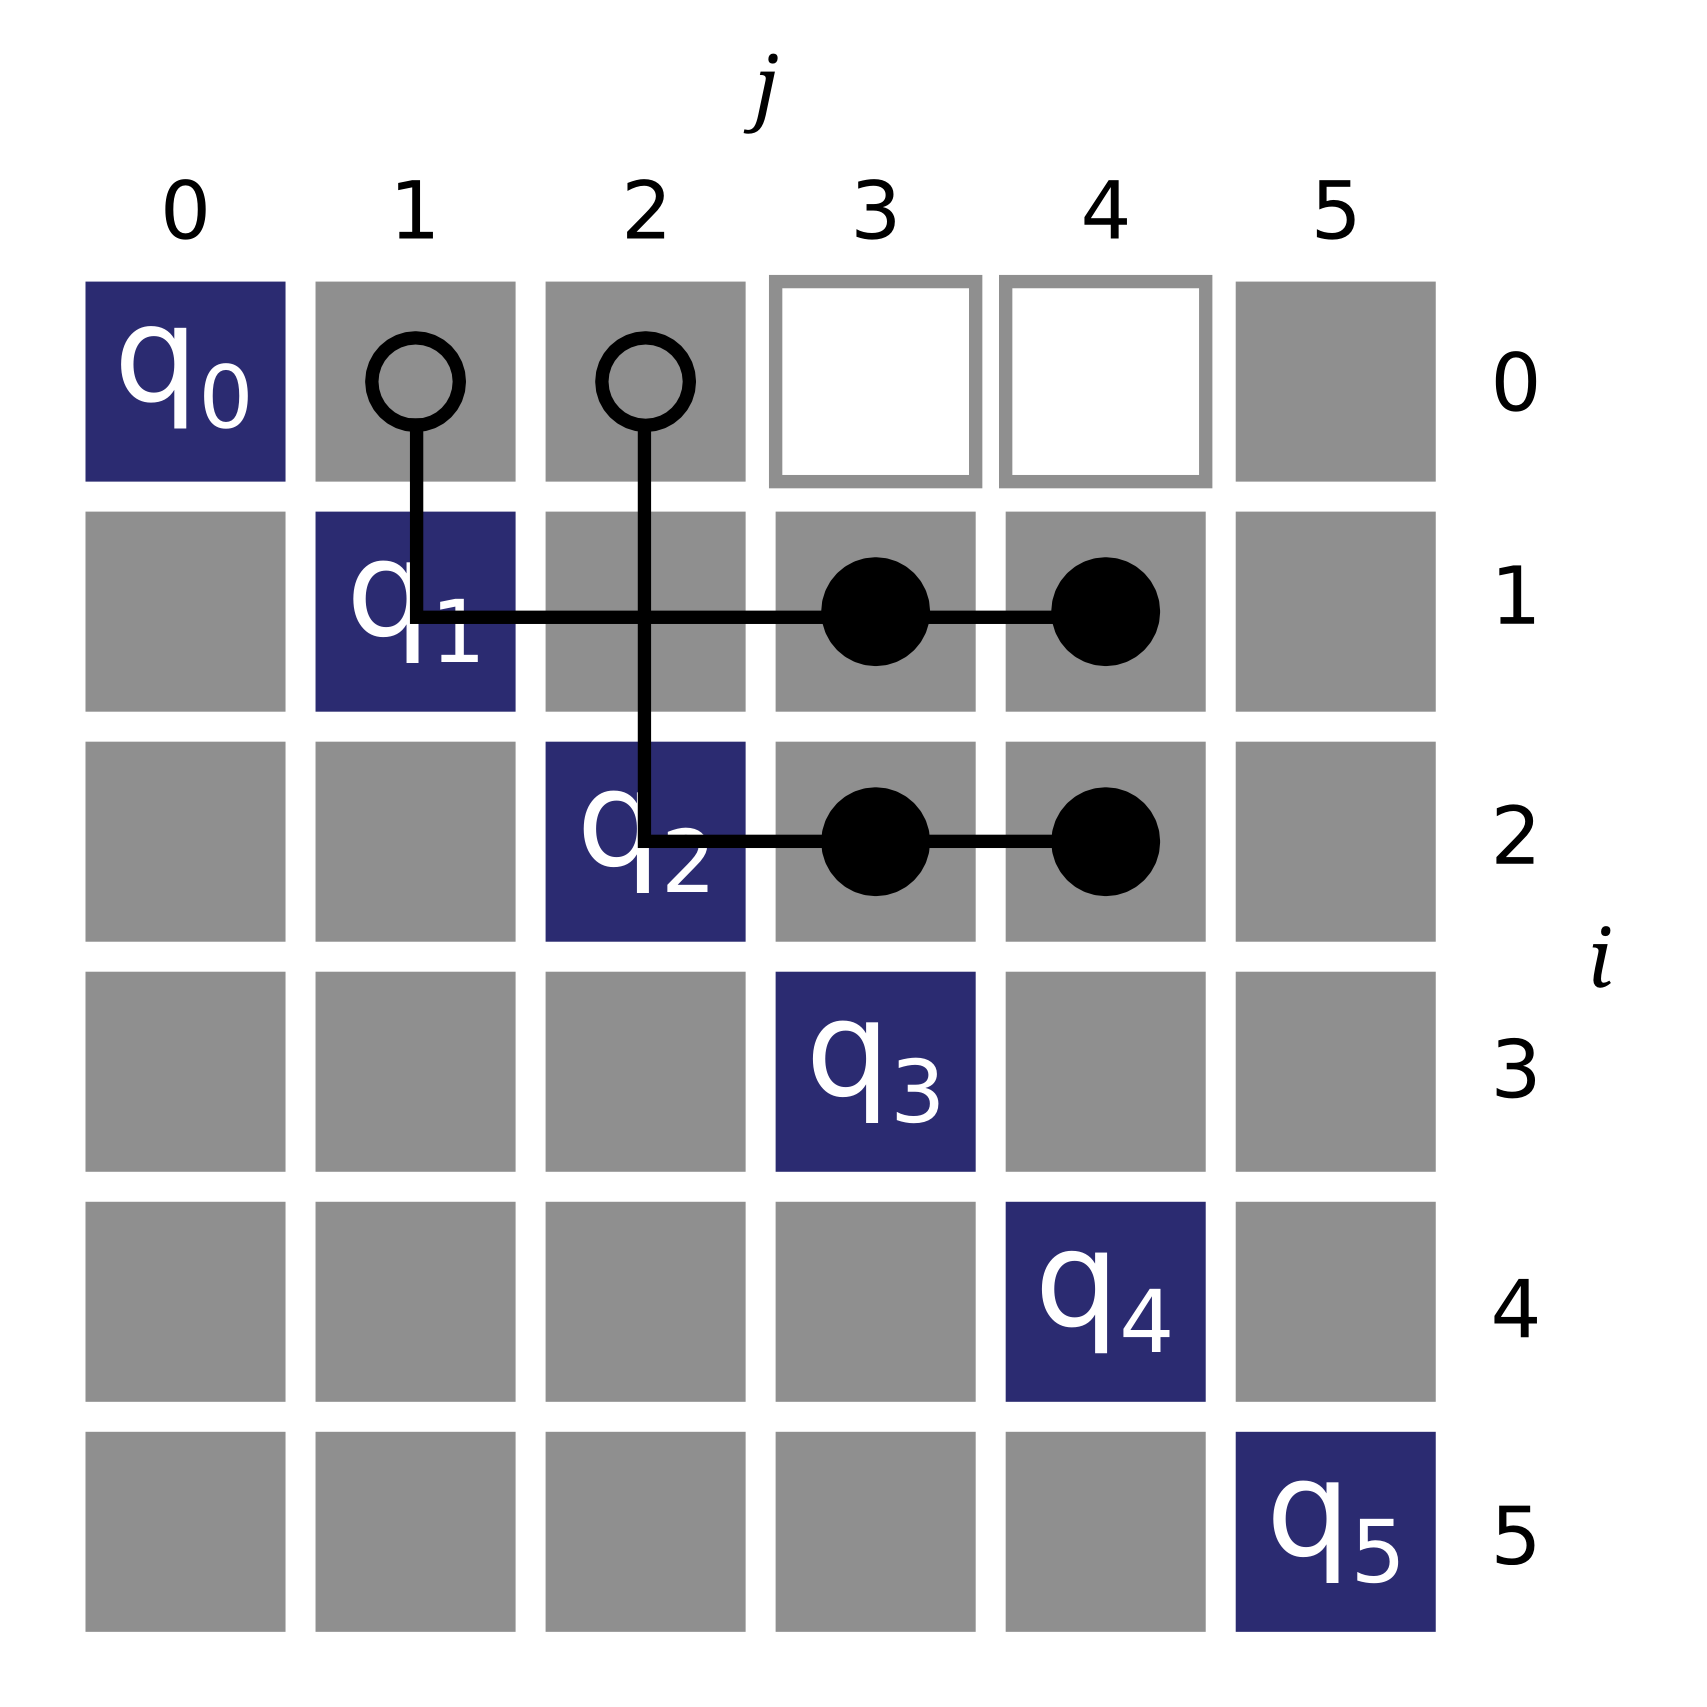
\includegraphics[width=0.33\textwidth]{img/vectorized_blocking.png}
  \caption{Vectorization of Partial Results.\label{fig:vec-blocking}}
\end{figure}

\mypar{Vectorized Blocking} Once we properly implemented blocking, it is
straight-forward to apply vectorization.

\section{Experimental Results}


\begin{figure}\centering
  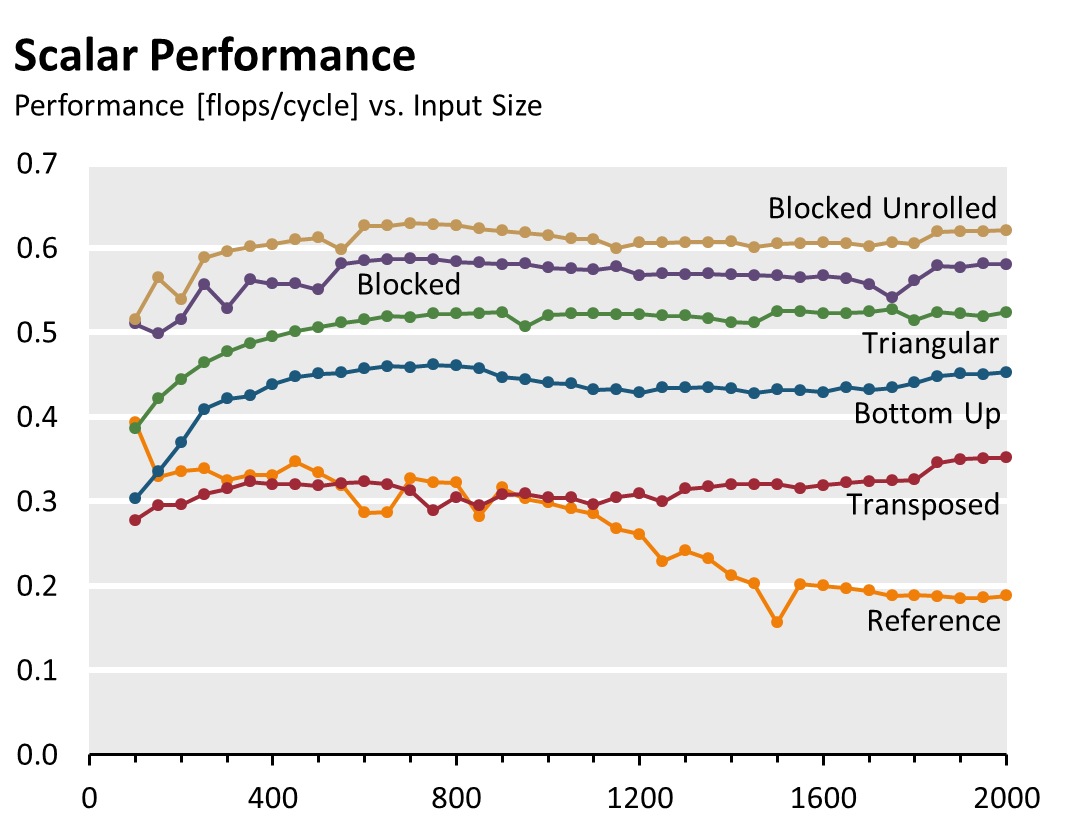
\includegraphics[width=\linewidth]{plot_data/scalar_performance.png}
  \caption{One code to rule 'em all.}
  \label{fig:perf-scalar}
\end{figure}
\begin{figure}\centering
  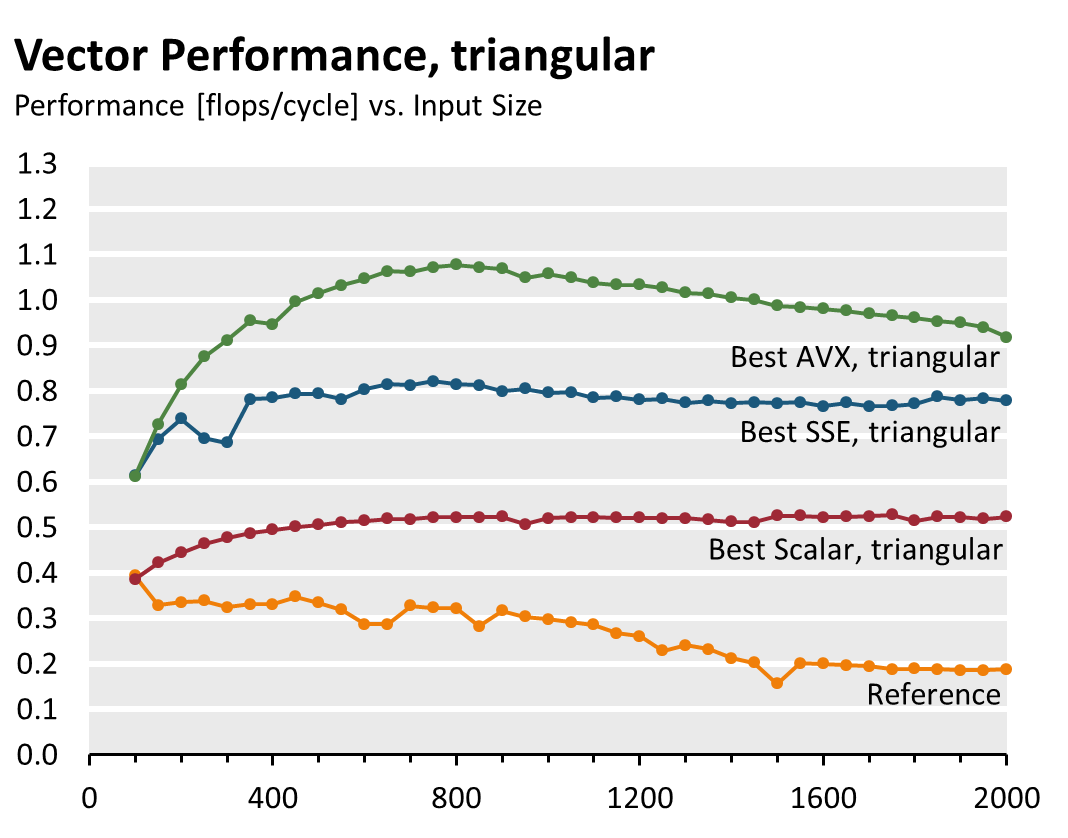
\includegraphics[width=\linewidth]{plot_data/triangular_vector_performance.png}
  \caption{One code to rule 'em all.}
  \label{fig:perf-triangular}
\end{figure}
\begin{figure}\centering
  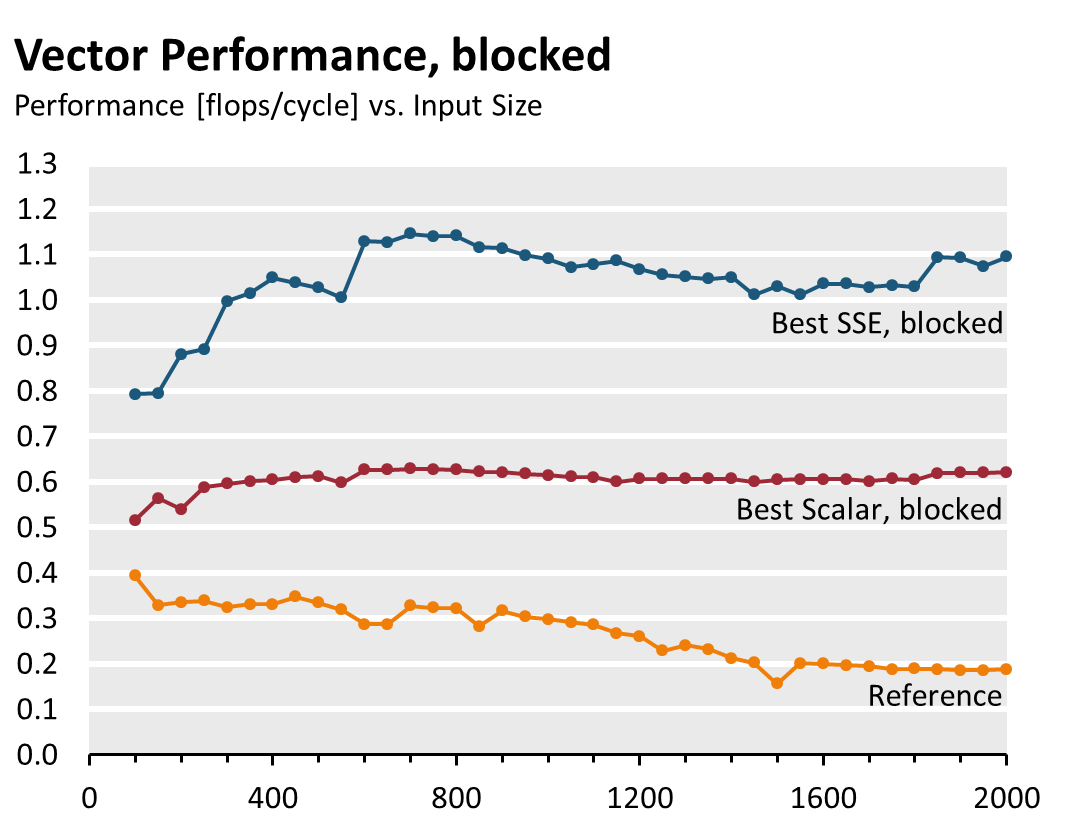
\includegraphics[width=\linewidth]{plot_data/blocked_vector_performance.png}
  \caption{One code to rule 'em all.}
  \label{fig:perf-blocked}
\end{figure}
\begin{figure}\centering
  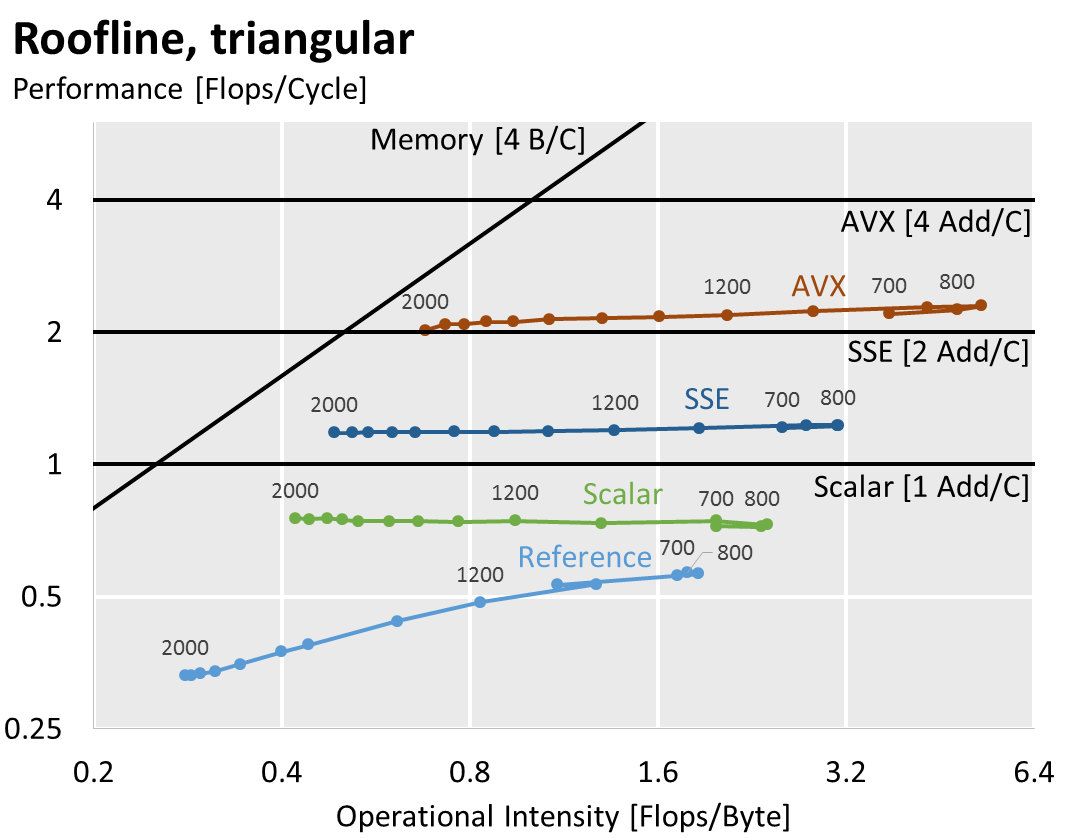
\includegraphics[width=\linewidth]{roofline-data/roofline_triangular.png}
  \caption{One code to rule 'em all.}
  \label{fig:roofline-triangular}
\end{figure}
\begin{figure}\centering
  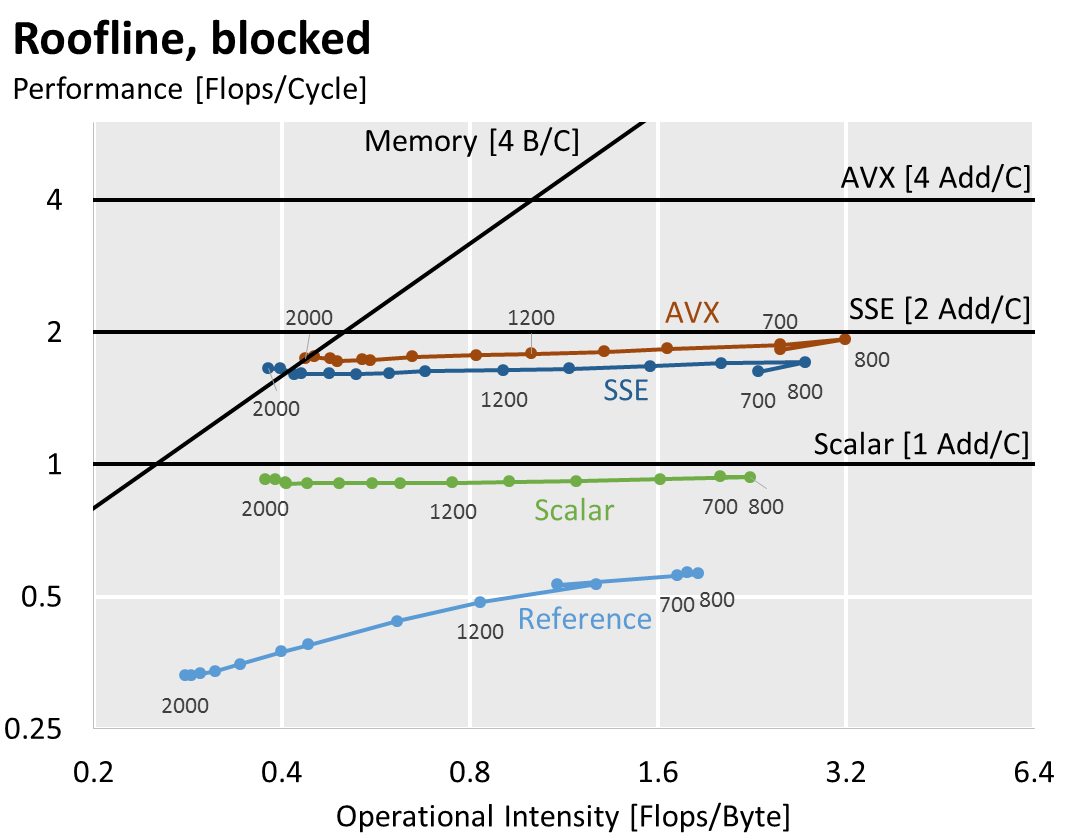
\includegraphics[width=\linewidth]{roofline-data/roofline_blocked.png}
  \caption{One code to rule 'em all.}
  \label{fig:roofline-blocked}
\end{figure}

\section{Conclusions}


\appendix


The hard page limit is 6 pages in this style. Do not reduce font size
or use other tricks to squeeze. This pdf is formatted in the American letter format, so may look a bit strange when printed out.

\begin{abstract}
Describe in concise words what you do, why you do it (not necessarily
in this order), and the main result.  The abstract has to be
self-contained and readable for a person in the general area. You
should write the abstract last.
\end{abstract}

\section{Introduction}

Do not start the introduction with the abstract or a slightly modified
version. It follows a possible structure of the introduction.
Note that the structure can be modified, but the
content should be the same. Introduction and abstract should fill at most the first page, better less.

\mypar{Motivation} The first task is to motivate what you do.  You can
start general and zoom in one the specific problem you consider.  In
the process you should have explained to the reader: what you are doing,
why you are doing, why it is important (order is usually reversed).

For example, if my result is the fastest DFT implementation ever, one
could roughly go as follows. First explain why the DFT is important
(used everywhere with a few examples) and why performance matters (large datasets,
realtime). Then explain that fast implementations are very hard and
expensive to get (memory hierarchy, vector, parallel). 

Now you state what you do in this paper. In our example: 
presenting a DFT implementation that is
faster for some sizes than all the other ones.

\mypar{Related work} Next, you have to give a brief overview of
related work. For a paper like this, anywhere between 2 and 8
references. Briefly explain what they do. In the end contrast to what
you do to make now precisely clear what your contribution is.

\section{Background: Whatever the Background is}\label{sec:background}

Give a short, self-contained summary of necessary
background information. For example, assume you present an
implementation of FFT algorithms. You could organize into DFT
definition, FFTs considered, and cost analysis. The goal of the
background section is to make the paper self-contained for an audience
as large as possible. As in every section
you start with a very brief overview of the section. Here it could be as follows: In this section 
we formally define the discrete Fourier transform, introduce the algorithms we use
and perform a cost analysis.

\mypar{Discrete Fourier Transform}
Precisely define the transform so I understand it even if I have never
seen it before.

\mypar{Fast Fourier Transforms}
Explain the algorithm you use.

\mypar{Cost Analysis}
First define you cost measure (what you count) and then compute the
cost. Ideally precisely, at least asymptotically. In the latter case you will need to instrument your code to count
the operations so you can create a performance plot.

Also state what is
known about the complexity (asymptotic usually) 
about your problem (including citations).

Don't talk about "the complexity of the algorithm.'' It's incorrect,
remember (Lecture 2)?


\section{Your Proposed Method}\label{sec:yourmethod}

Now comes the ``beef'' of the paper, where you explain what you
did. Again, organize it in paragraphs with titles. As in every section
you start with a very brief overview of the section.

For this class, explain all the optimizations you performed. This mean, you first very briefly
explain the baseline implementation, then go through locality and other optimizations, and finally SSE (every project will be slightly different of course). Show or mention relevant analysis or assumptions. A few examples: 1) Profiling may lead you to optimize one part first; 2) bandwidth plus data transfer analysis may show that it is memory bound; 3) it may be too hard to implement the algorithm in full generality: make assumptions and state them (e.g., we assume $n$ is divisible by 4; or, we consider only one type of input image); 4) explain how certain data accesses have poor locality. Generally, any type of analysis adds value to your work.

As important as the final results is to show that you took a structured, organized approach to the optimization and that you explain why you did what you did.

Mention and cite any external resources including library or other code.

Good visuals or even brief code snippets to illustrate what you did are good. Pasting large amounts of code to fill the space is not good.

\section{Experimental Results}\label{sec:exp}

Here you evaluate your work using experiments. You start again with a
very short summary of the section. The typical structure follows.

\mypar{Experimental setup} Specify the platform (processor, frequency, cache sizes)
as well as the compiler, version, and flags used. I strongly recommend that you play with optimization flags and consider also icc for additional potential speedup.

Then explain what input you used and what range of sizes. The idea is to give enough information so the experiments are reproducible by somebody else on his or her code.

\mypar{Results}
Next divide the experiments into classes, one paragraph for each. In the simplest case you have one plot that has the size on the x-axis and the performance on the y-axis. The plot will contain several lines, one for each relevant code version. Discuss the plot and extract the overall performance gain from baseline to best code. Also state the percentage of peak performance for the best code. Note that the peak may change depending on the situation. For example, if you only do additions it would be 12 Gflop/s
on one core with 3 Ghz and SSE and single precision floating point.

Do not put two performance lines into the same plot if the operations count changed significantly (that's apples and oranges). In that case first perform the optimizations that reduce op count and report the runtime gain in a plot. Then continue to optimize the best version and show performance plots.

{\bf You should}
\begin{itemize}
\item Follow the guide to benchmarking presented in class, in particular
\item very readable, attractive plots (do 1 column, not 2 column plots
for this class), proper readable font size. An example is below (of course you can have a different style),
\item every plot answers a question, which you pose and extract the
answer from the plot in its discussion
\end{itemize}
Every plot should be discussed (what does it show, which statements do
you extract).

\section{Conclusions}

Here you need to briefly summarize what you did and why this is
important. {\em Do not take the abstract} and put it in the past
tense. Remember, now the reader has (hopefully) read the paper, so it
is a very different situation from the abstract. Try to highlight
important results and say the things you really want to get across
(e.g., the results show that we are within 2x of the optimal performance ... 
Even though we only considered the DFT, our optimization
techniques should be also applicable ....) You can also formulate next
steps if you want. Be brief.

\section{Further comments}

Here we provide some further tips.

\mypar{Further general guidelines}

\begin{itemize}
\item For short papers, to save space, I use paragraph titles instead of
subsections, as shown in the introduction.

\item It is generally a good idea to break sections into such smaller
units for readability and since it helps you to (visually) structure the story.

\item The above section titles should be adapted to more precisely
reflect what you do.

\item Each section should be started with a very
short summary of what the reader can expect in this section. Nothing
more awkward as when the story starts and one does not know what the
direction is or the goal.

\item Make sure you define every acronym you use, no matter how
convinced you are the reader knows it.

\item Always spell-check before you submit (to me in this case).

\item Be picky. When writing a paper you should always strive for very
high quality. Many people may read it and the quality makes a big difference.
In this class, the quality is part of the grade.

\item Books helping you to write better: \cite{Higham:98} and \cite{Strunk:00}.

\item Conversion to pdf (latex users only): 

dvips -o conference.ps -t letter -Ppdf -G0 conference.dvi

and then

ps2pdf conference.ps
\end{itemize}

\mypar{Graphics} For plots that are not images {\em never} generate (even as intermediate step)
jpeg, gif, bmp, tif. Use eps, which means encapsulate postscript, os pdf. This way it is
scalable since it is a vector graphic description of your graph. E.g.,
from Matlab, you can export to eps or pdf.

Here is an example of how to get a plot into latex.
Note that the text should not be any smaller than shown.
You might also like \autoref{fig:scalar}.

\begin{figure}\centering
  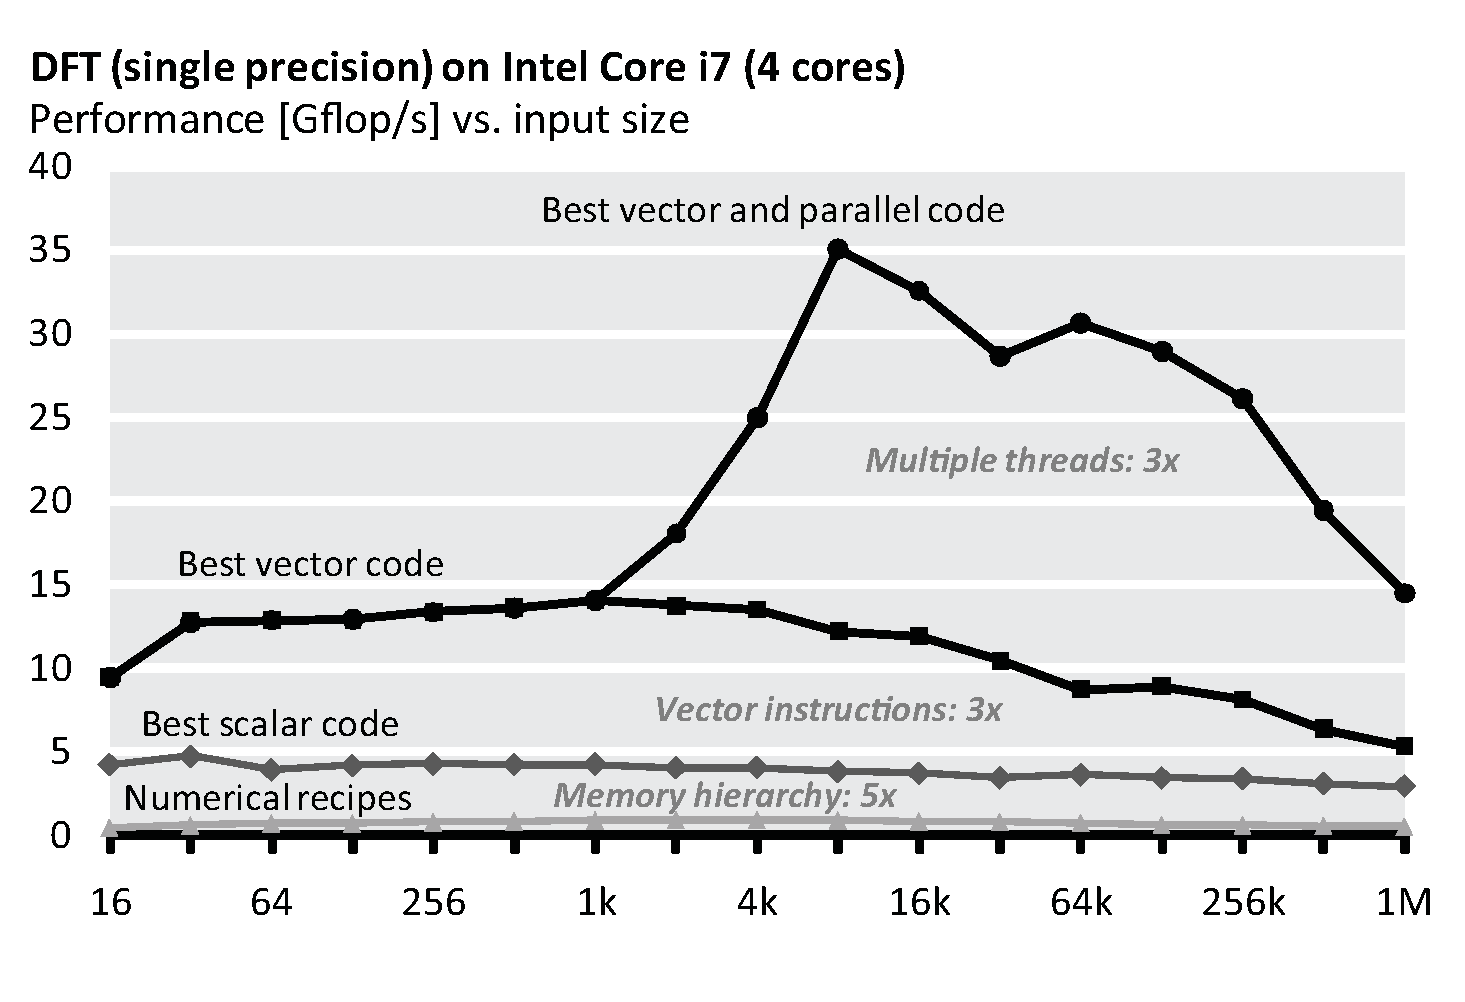
\includegraphics[width=\linewidth]{dft-performance.eps}
  \caption{foo}
  \label{foo}
\end{figure}

\begin{figure}\centering
  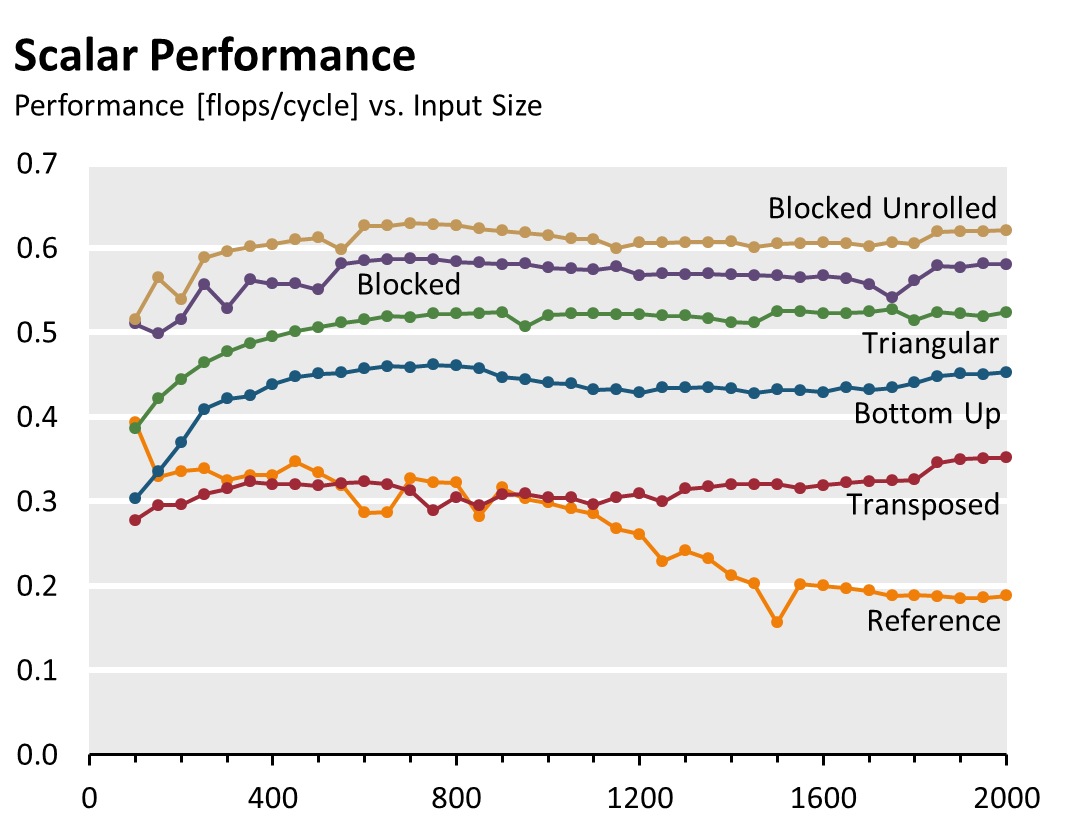
\includegraphics[width=\linewidth]{plot_data/scalar_performance.png}
  \caption{One code to rule 'em all.}
  \label{fig:perf-scalar}
\end{figure}
\begin{figure}\centering
  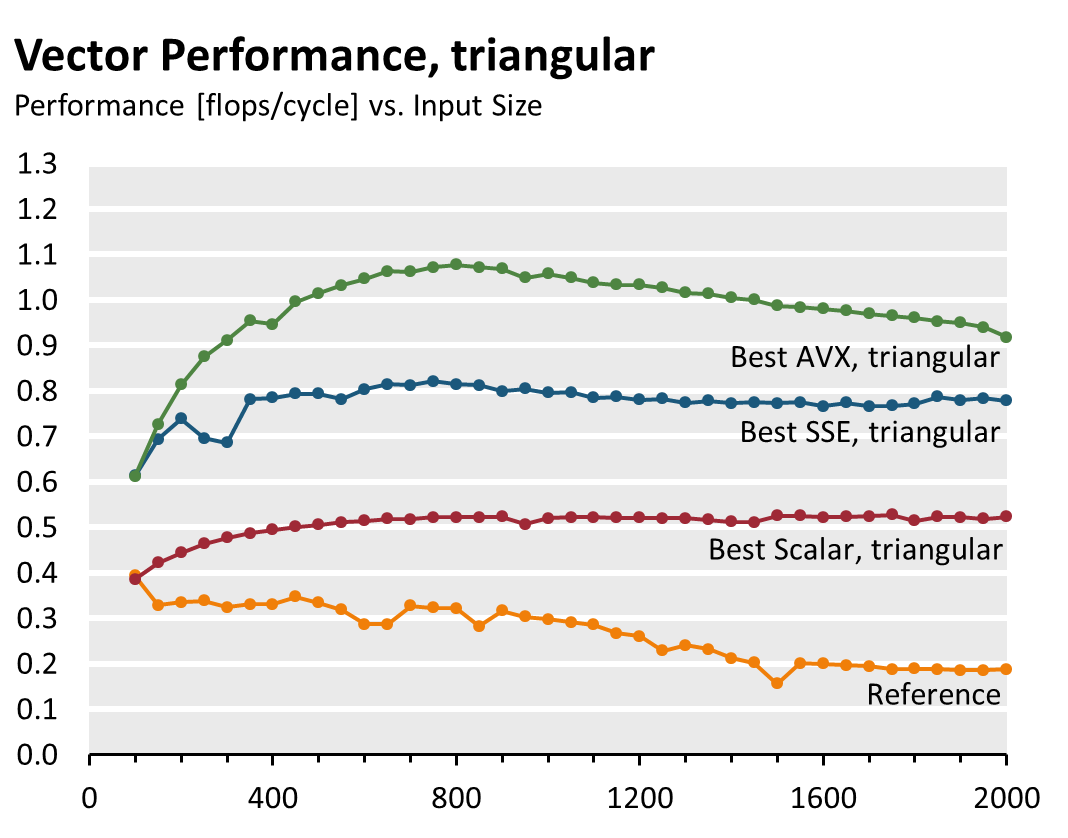
\includegraphics[width=\linewidth]{plot_data/triangular_vector_performance.png}
  \caption{One code to rule 'em all.}
  \label{fig:perf-triangular}
\end{figure}
\begin{figure}\centering
  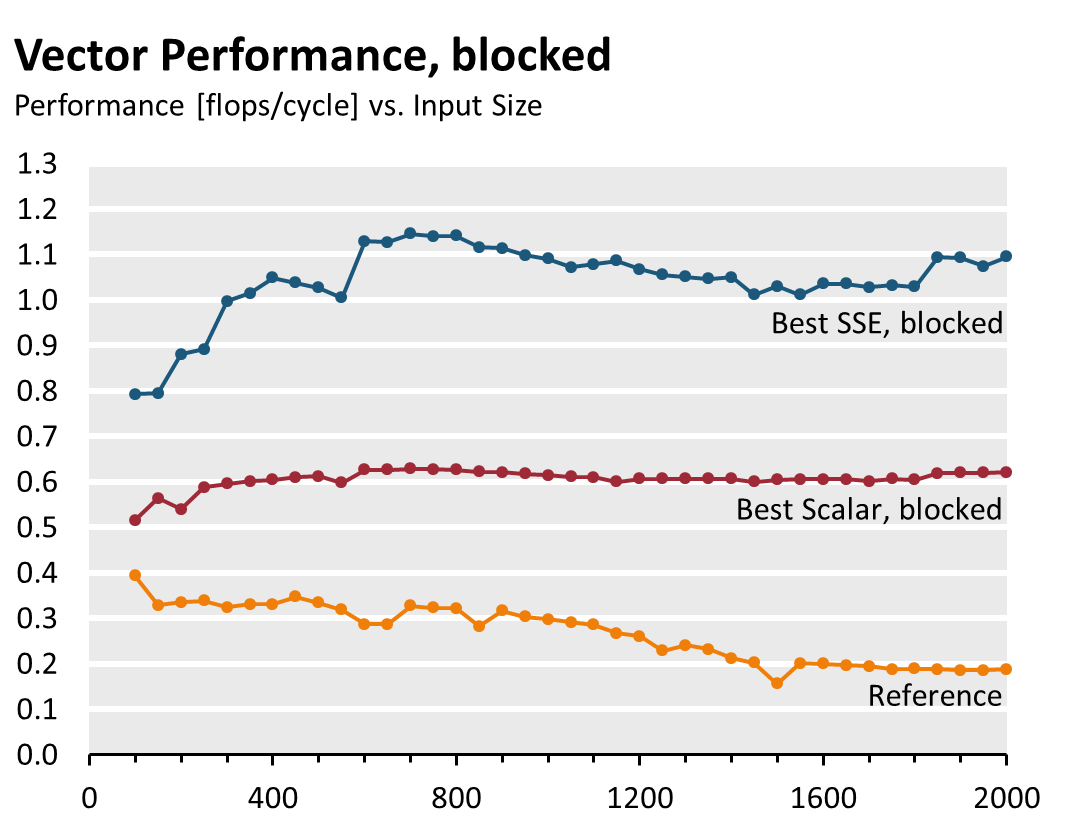
\includegraphics[width=\linewidth]{plot_data/blocked_vector_performance.png}
  \caption{One code to rule 'em all.}
  \label{fig:perf-blocked}
\end{figure}



% References should be produced using the bibtex program from suitable
% BiBTeX files (here: bibl_conf). The IEEEbib.bst bibliography
% style file from IEEE produces unsorted bibliography list.
% -------------------------------------------------------------------------
\bibliographystyle{IEEEbib}
\bibliography{bibl_conf}

\end{document}

